\documentclass[11pt]{article}
\usepackage[a4paper,margin=2.7cm]{geometry}
\usepackage{amsmath,amssymb}
\usepackage{graphicx}
\usepackage{booktabs}
\usepackage[round]{natbib}
\usepackage[colorlinks=true,linkcolor=blue!60!black,citecolor=blue!60!black,urlcolor=blue!60!black]{hyperref}
\usepackage{xcolor}

\graphicspath{{figs/}}
\newcommand{\astar}{\alpha^{*}}

\title{Message capacity and claim wording set the transition points of collective truth-finding in language-model networks}
\author{Makoto Fukushima\thanks{Honda Research Institute Japan.
Email: \texttt{makoto.fukushima@jp.honda-ri.com}}}
\date{}

\begin{document}
\maketitle

\begin{abstract}
Whether human or large language model (LLM), an agent in discussion
processes only a few of the others' contributions, bounded by cognition,
context, or cost.
LLM collectives can settle on a wrong consensus even from a correct majority;
we ask how far that bound alone fixes their fate, as crowding parameter
$\alpha$: each agent accepts an input with probability $e^{-\alpha r}$
after $r$ acceptances. Over 31{,}824 randomized queries,
we found that an 8-billion-parameter model's judgment of a claim effectively
reduces to a logistic function of a weighted sum of its inbox, equivalent to a
stochastic binary neuron with divisively normalized weights. From these
coefficients and degree statistics alone, the wrong-consensus basin should
vanish at $\astar = 0.435$ (6.4 of 31 sources). In 1{,}414 episodes
with assigned opinions the prediction failed: correct-side outcomes stayed
below 50\% of episodes from every start, 28--45\% from 75\%-correct
majorities. The failure traces to the field, the tilt each claim's wording
induces: the experimental claims' fields lay below the calibration mean;
with each claim's own field the same weights reproduce the outcomes.
Reversing the wording showed the tilt follows a claim's assertion, not its
truth. On a
second 8B model the pipeline predicts claim-dependent bistability; basin
boundaries appeared where computed, and eight-claim calibration matched in
15 of 16 conditions. At 70B the assertion bias is not detected.
A collective's fate is thus largely set by two single-agent
measurements: the tilt a claim's wording induces, and the message capacity
that sets the transition point.
\end{abstract}

\section*{Significance statement}

Language-model agents are beginning to operate in groups that debate and
settle on answers, and such groups can talk themselves into the wrong one.
This work shows that a group's fate is largely set by two quantities
measurable on a single agent. An agent's judgment reduces to the input-output
rule of a stochastic binary neuron with divisively normalized inputs, so the
group's transition point follows, through a reduced map, from how many
sources each member reads; the second quantity is the tilt a claim's wording
induces on each reading. Across three models, collectives followed the
assertion rather than the truth in one and crossed predicted transition
points in another. AI
collectives can be assessed, and designed, before they run.

\section{Introduction}\label{sec:intro}

Groups of LLM agents that exchange messages and update binary opinions are now
studied as statistical-mechanical systems. \citet{El2026} showed that a kinetic
Ising model fitted to one-step transitions describes more than 10{,}000 such communities
($N = 32$, eight rounds), predicts individual trajectories, and generalizes to
unseen communication graphs. In that framework, as in most multi-agent opinion
studies, the interaction graph is supplied by the experimenter; the question of
where the graph comes from, and what its statistics do to the collective
outcome, is listed by those authors as future work.

A separate line of work on synaptic resource allocation provides a
one-parameter answer to the first half of that question. If a receiving unit
accepts a further input with probability $e^{-\alpha r}$ once $r$ inputs are
already accepted, the number of accepted inputs grows only logarithmically in
the candidate pool: the mean in-degree is $(\log N)/\alpha$ with bounded
variance, the full in-degree distribution $P_{\alpha,N}(k)$ obeys a closed
recursion, and the distribution is invariant under reordering of the
candidates \citep{SciRepCrowding}. The parameter $\alpha$ --- the crowding
parameter --- compresses everything about the acceptance process that matters
for degree statistics. Throughout, $\alpha$ describes the crowding of a finite intake budget, the message capacity of an agent, at the level of whole messages; it is unrelated to the attention
mechanism inside transformer architectures, and we avoid the word ``attention'' for this reason.

The bound itself is not particular to machines. Human deliberation operates under cognitive limits of the same shape: working memory holds only a few items at once \citep{Cowan2001}, and divided attention caps how many contributions a participant actually processes \citep{HodasLerman2012}. A theory that turns an intake bound into a collective outcome is, at least potentially, a statement about committees and juries as well as about machine collectives. In human groups, however, neither the bound nor the network it induces can be measured or controlled; in LLM collectives, both can.

These two ingredients suggest a quantitative question. Consider a population
in which a fraction $x_0$ of agents initially holds the correct answer to a
binary question. After several rounds of exchange the population typically
reaches a correct or a wrong consensus; the probability of the former after
a fixed number of rounds, $q(x_0)$, is the finite-horizon analogue of the
committor of the collective dynamics (Methods). Mean-field theory on
the generated networks predicts that the basin of the wrong consensus
disappears entirely above a critical crowding level $\astar$: for
$\alpha > \astar$, even small correct minorities propagate. Our question is to
what extent $\astar$ can be computed in advance --- from the degree statistics
that $\alpha$ induces and from response coefficients measured on single agents
in isolation --- with no quantity fitted to collective runs. The nearest precedents come from LLM naming games, where emergent
conventions and collective bias are established phenomena
\citep{Ashery2025, Flint2026}: a mean-field consensus condition has been
assembled from single-token acceptance rates measured on isolated models
\citep{DeNobili2026}, and a mean-field account of population-size-dependent
collective bias from logit-extracted single-agent policies
\citep{Flint2026}. These constructions share our logic, but they concern
coordination on a convention (no correct side, no committor) under
fully mixed or imposed interaction structures. No previous study has, to our knowledge,
generated the interaction network of an LLM collective from a crowding
process, or predicted the basin boundary of a truth-finding collective ---
the critical initial fraction of correct agents --- from single-agent
measurements completed before the collective ran.

Two families of confound make this comparison easy to get wrong, and both have
shaped our design. First, in observational data the initial fraction $x_0$ is
not an experimental dial: we show in Section~\ref{sec:reanalysis} that in the
largest public dataset $x_0$ is driven by question difficulty, which also
drives the outcome, so the apparent committor is a difficulty curve and the transition point (the tipping point of the social-dynamics literature) is unidentified. Our collective experiment therefore assigns
initial opinions exogenously. Second, changing the network changes the
composition of each agent's prompt, and LLMs respond to prompt composition
regardless of any network; effects of this kind reproduce in a single agent
with a single query. We therefore measure the single-agent response function
first (Section~\ref{sec:measurement}), predict the collective outcome from it,
and treat any residual --- quantified by replaying every realized prompt
through the measured response function --- as the collective contribution proper.

The paper proceeds in three steps: a theory of $\astar$ from a reduced map
(Section~\ref{sec:theory}), the measurements that reduce the experimental agent to a stochastic binary neuron and give the theory its empirical coefficients (Sections~\ref{sec:reanalysis}--\ref{sec:measurement}), and a
collective experiment run against the pre-registered prediction
(Section~\ref{sec:collective}). The pre-registered prediction fails, and the
failure is traced to two measurable causes rather than to the collective
step: the tilt each claim's wording induces (its field), which did not carry
over from the calibration claims to the experimental ones, and the
eight-round horizon, which is short
against the relaxation of the mean-field map near its fold. Two further
campaigns then identify what dominated: an assertion-polarity bias specific
to the model class, established by a pre-registered discrimination experiment
and not shared by a second model --- and in that second model the same
pipeline predicts claim-dependent bistability whose basin boundaries are
observed at the computed positions. To what extent a collective's truth-finding is
decided by individual input crowding is, on this evidence, a question with a
computable answer --- model by model, claim by claim.

\begin{figure}[t]
\centering
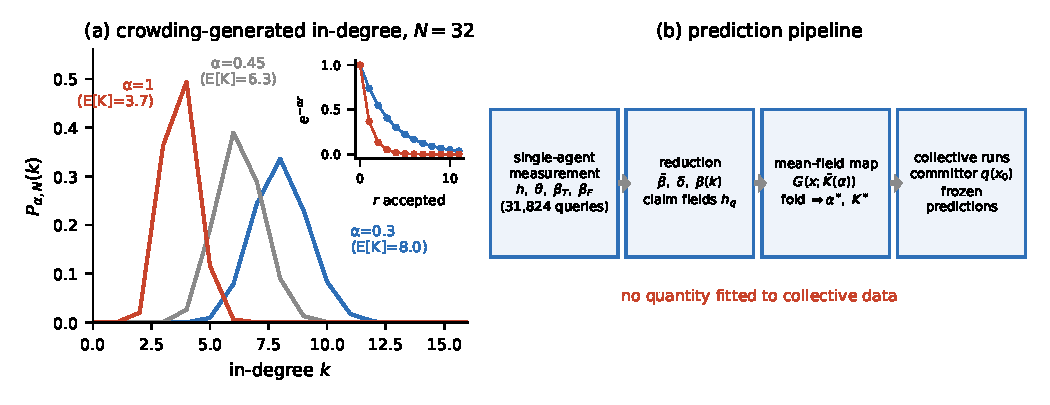
\includegraphics[width=\textwidth]{fig1_framework}
\caption{\textbf{Crowding-generated networks and the prediction pipeline.}
(a)~In-degree distribution $P_{\alpha,N}(k)$ generated by the acceptance
process $e^{-\alpha r}$ (inset) at three crowding levels, $N=32$.
(b)~Every quantity used to predict the collective outcome is measured on
single agents or computed from the reduced map; nothing is fitted to
collective data.}
\label{fig:framework}
\end{figure}

\section{Theory: a critical crowding level from a reduced map}\label{sec:theory}

\subsection{Network generation}

The generation process and its degree statistics are those of
\citet{SciRepCrowding}: each receiving agent processes the other $N-1$
agents in arbitrary order and, having already accepted $r$ sources, accepts
the next with probability $e^{-\alpha r}$ (the first is always accepted);
the in-degree distribution $P_{\alpha,N}(k)$ follows the recursion
$P_{m+1}(r) = P_m(r)\,(1-e^{-\alpha r}) + P_m(r-1)\,e^{-\alpha (r-1)}$,
with mean $E[K] = (\log N)/\alpha + O(1)$. New here is only the closure:
the deterministic continuum limit gives the finite-$N$ form
\begin{equation}
\bar K(\alpha) = \frac{1}{\alpha}\,\ln\!\bigl(1 + \alpha (N-1)\bigr),
\end{equation}
which underestimates the exact mean by 3\% ($\alpha = 0.3$) to 11\%
($\alpha = 2$) at $N = 32$; where precision matters we invert the exact
recursion instead. Eq.~(1) is a large-$N$, moderate-$\alpha$ form: as
$\alpha \to \infty$ it tends to zero, whereas the exact mean tends to one
because the first candidate is always accepted. Degree statistics are invariant under candidate reordering,
so manipulations of \emph{who} is read change nothing in $P(k)$ --- the
property that lets order-based conditions be compared at exactly matched
communication budgets.

\subsection{Single-agent response and its reduction}

Measurements in Section~\ref{sec:measurement} show that an agent receiving $l$
correct-side and $k-l$ wrong-side messages adopts the correct side with
probability
$\sigma(c_0 + \theta\,\mathbf{1}[\text{own state correct}] + \beta_T l +
\beta_F (k-l))$, where $\sigma$ is the logistic function (with the per-message weights attenuated by inbox size as $\beta g(k)$; Section~\ref{sec:measurement}); the measured unit is equivalent to a stochastic binary neuron. Three combinations
organize everything that follows: the symmetry-breaking field
$h = c_0 + \theta/2$, the tilt that the claim's wording induces on each
reading, measured per claim (the persistence indicator decomposes into a
constant field $\theta/2$ plus a symmetric term), the per-input swing
$\bar\beta = (\beta_T - \beta_F)/2$, and the per-input drift
$\delta = (\beta_T + \beta_F)/2$.
The population dynamics under heterogeneous mean field (HMF) --- each of an
agent's $k$ inputs correct independently with probability $x$ --- is the
one-dimensional map
\begin{equation}
F(x) = \sum_{k} P_{\alpha,N}(k) \sum_{l=0}^{k} \binom{k}{l}
x^{l} (1-x)^{k-l} \bigl[\, x\,\sigma(u_{1}) + (1-x)\,\sigma(u_{0})
\bigr],
\label{eq:hmfmap}
\end{equation}
with $u_{s} = c_0 + \theta s + \beta_T l + \beta_F (k-l)$; the interior
unstable fixed point of $F$ separates the two consensus basins. The
construction is the mean-field analysis of the generating model
\citep{SciRepCrowding} with one substitution: the hard-threshold unit
assumed there is replaced by the measured logistic unit, of which the
threshold unit is the infinite-gain limit; the outcome observable
$q(x_0)$ is likewise inherited from that analysis, which computed the
committor proper by an absorbing Markov-chain closure; here it is read after
eight rounds (Methods). No threshold
nonlinearity is assumed anywhere below --- bistability is a property of the
fixed-point structure of the S-shaped map, an unstable interior fixed point
separating two stable ones --- and the substitution
removes the structural discontinuity that hard-threshold updates produce at truth-weight 1 (equal per-message weight for correct-side and wrong-side sources; Section~\ref{sec:reanalysis}). Exact numerics iterate
Eq.~(\ref{eq:hmfmap}) directly; closing the degree at $\bar K(\alpha)$ and
smoothing the binomial with the standard Gaussian--logistic approximation
yields the reduced map
\begin{equation}
G(x;K) = x\,\sigma(z_+) + (1-x)\,\sigma(z_0), \qquad
z_s = \frac{(h \pm \theta/2) + K\delta + 2\bar\beta K (x - \tfrac12)}
{\sqrt{1 + \tfrac{\pi}{8}\, 4\bar\beta^2 K x(1-x)}}.
\end{equation}
A degree-dependent coupling $g(k)$, for example the divisive normalization
$\beta/(1+\gamma k)$, one of the two attenuation forms our data support,
enters by multiplying $\bar\beta$ and $\delta$, leaving the form unchanged.

\subsection{The critical capacity}\label{sec:critical}

$\astar$ is the capacity at which the interior unstable fixed point of $G$
undergoes a fold ($G = x$ and $G' = 1$ simultaneously). We keep the term
critical crowding level for $\astar$ for continuity with the generating
model, but the transition is a saddle-node bifurcation of the mean-field
map, corresponding to the disappearance of a metastable basin (a spinodal);
the Discussion returns to the distinction. Operationally: the
fold defines a threshold degree $K^*$, and $\astar$ solves
$\bar K(\alpha) = K^*$. The mechanism is visible in the linear gain at the
symmetric point,
\begin{equation}
\lambda(K) = \bigl[\sigma(z_+) - \sigma(z_0)\bigr]
+ \frac{2\bar\beta K\,\bar\sigma'}{\sqrt{1 + \tfrac{\pi}{8}\bar\beta^2 K}},
\end{equation}
a persistence gain (first term, carried by $\theta$) plus a
social-amplification gain that, for constant coupling, grows only as
$\sqrt{K}$ because input fluctuations smooth the response; here
$\bar\sigma' = [\sigma'(z_+) + \sigma'(z_0)]/2$, with every term evaluated at
$x = 1/2$. In the symmetric case ($h = 0$ and $\delta = 0$) bistability requires $\lambda > 1$.
With a nonzero field the gain at the symmetric point locates the mechanism
but is neither necessary nor sufficient for bistability, and it misplaces
$\astar$ by 30--90\% at realistic fields, so all quantitative predictions
below come from the fold of $G$. One further structural fact falls out of the
reduction: with the measured $\delta < 0$ the effective field
$h + K\delta\,g(K)$ is screened as degree grows (with constant coupling it
crosses zero near $K \approx 10$ for the coefficients measured in
Section~\ref{sec:measurement} under the collective experiment's prompt,
variant A), which is why bistability survives at low $\alpha$ despite
$h > 0$. Under divisive coupling this screening saturates: $K\delta\,g(K)
\to \delta/\gamma$, and over the mean degrees realized here ($K \approx 3$--$10$)
the factor $K g(K)$ varies only between 0.82 and 1.0, so the effective field, and
with it the threshold position, depends only weakly on $\alpha$. The weak
$\alpha$-dependence of the qwen3:8b thresholds (Section~\ref{sec:generality})
is consistent with this; the zero crossing itself is not tested separately.

Against exact numerics (the full $P(k)$ sum, fold located by bisection in
$\alpha$) the closure is accurate to a median 2.7\% over a 3-decade
parameter grid and both measured coefficient sets when the exact $E[K]$ is
inverted, and 6.7\% in the fully closed form; the worst cases are 6.0\%
(exact $E[K]$; the synthetic set $h = 0.7$, $\theta = 0.6$, $\bar\beta = 1$)
and 9.9\% (closed form; $h = 0.3$, $\theta = 2$, $\bar\beta = 1$)
(Fig.~\ref{fig:theory}; SI). For the measured variant-A
coefficients the prediction is $\astar = 0.435$, $K^* = 6.4$, as registered
(the fold conditions solved to full precision give 0.439 and $K^* = 6.36$,
inside the registered tolerance): the wrong-consensus basin is predicted to
disappear when agents accept, on average, fewer than 6.4 of their 31 possible
sources. The critical crowding level of the collective is, to this accuracy,
computable from single-agent coefficients through the reduced map.

\begin{figure}[t]
\centering
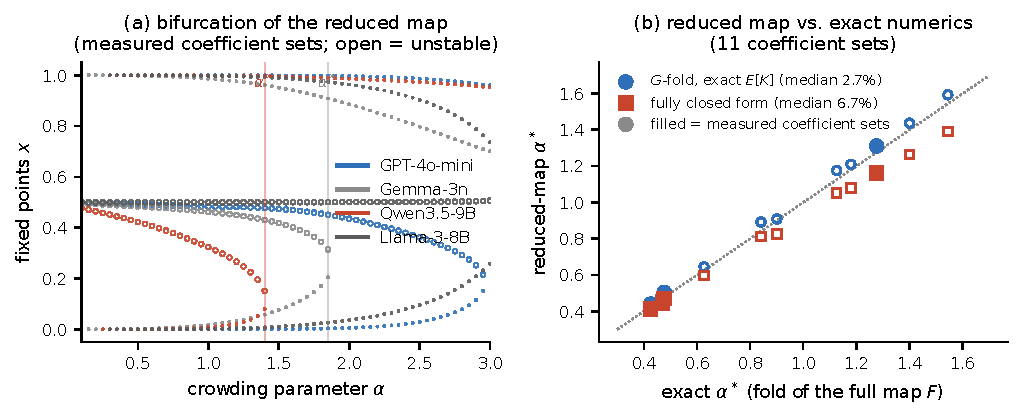
\includegraphics[width=\textwidth]{fig2_theory}
\caption{\textbf{Critical crowding level from the reduced map.} (a)~Fixed points of the
reduced map $G$ as functions of $\alpha$ for the four measured coefficient
sets of \citet{El2026}; the interior unstable branch (open symbols) vanishes
at $\astar$. (b)~Validation of the two closure levels against the fold of
the full map $F$ over 11 coefficient sets (filled symbols: coefficient sets
measured in this study).}
\label{fig:theory}
\end{figure}

\section{Why public data cannot test the prediction}\label{sec:reanalysis}

The natural first test requires no new data: \citet{El2026} released full logs of 6{,}400
objective-question communities (four models, 40 questions, ten graphs per question, four episodes) \citep{El2026data}. We computed each community's correct-side fraction trajectory
$x(t)$ and asked whether the apparent committor $q(x_0)$ identifies a transition point.

It does not, for a reason that constrains observational designs in which the initial fraction is not assigned. Across the four models, between 50\% and
99.5\% of the variance of $x_0$ lies \emph{between questions}; within
questions the $x_0$--outcome correlation drops to 0.04--0.27. Communities at
$x_0 \approx 0.40$ on different questions run to opposite consensuses with
near certainty, while communities at $x_0 = 0.15$ on an easy question converge
correctly in 32 of 32 episodes. Question difficulty drives both the initial
fraction and the outcome; the pooled $q(x_0)$ curve is a difficulty curve, and
its 0.5-crossing is not a property of the collective dynamics. A
question-clustered bootstrap widens the apparent confidence intervals on the
fitted crossing by a factor of 4--10, after which no pairwise difference among
models or graph families is resolved. Two further obstacles are structural: the
released graphs have nearly degenerate degree distributions (random family
mass concentrated on $k = 2$--$4$; lattices), so the degree-statistics content
of any mean-field prediction is untestable; and under the hard-threshold
update rule assumed in earlier work the predicted crossing jumps
discontinuously at truth-weight 1, reducing the comparison to a single bit.
These are limitations of the identification strategy, not of the dataset's
quality --- the same logs support the message-level measurement below, which
is what makes the rest of this paper possible.

The logs do yield the microscopic coefficients. Regressing each agent's
next-round correctness on the composition of its inbox (43{,}500 observations
per model, question-clustered errors), the truth asymmetry $w_T$ --- the
relative per-message weight of correct-side sources, previously estimated at
1.16--1.71 from Ising couplings --- is indistinguishable from 1 in all four
models (e.g.\ GPT-4o-mini: 1.055, 95\% CI $[0.996, 1.114]$), while three other
coefficients are robustly nonzero: a persistence term $\theta$, an individual
field $c_0$, and an attenuation $\lambda_{\mathrm{lab}} = 0.08$--$0.56$ of
messages arriving through ``disagree''-labeled edges. The asymmetry that
breaks the symmetric degeneracy of the mean-field map therefore resides in the
field $h = c_0 + \theta/2$, not in message weighting --- which is what
Section~\ref{sec:theory} assumes. Public data fix the form of the theory; they
cannot test its collective prediction.

\section{Measuring the response function of the experimental agent}
\label{sec:measurement}

The collective experiment uses llama3.1:8b (4-bit Q4\_K\_M quantization, temperature 0.7,
snap-judgement prompt matching El et al.'s protocol). We measured its response
function directly: 31{,}824 single-shot queries in which the inbox composition
($k$ messages, $l$ of them correct-side), the A/B label assignment, the
message order, and an optional explicit own-state line were randomized by
design. Claims came from CLIMATE-FEVER \citep{Diggelmann2020}; a two-stage
calibration under the bare judgment prompt selected 17 claims with per-claim
field $|h_q| < 0.4$. Under the full experimental scaffold (persona and inbox
lines) the fields did not transfer: the per-claim intercepts re-expanded to a
range of 3.5 logits with mean 0.94, which is why the claims of the collective
experiment were calibrated again under the full scaffold (Methods), and why
the field, not the message weights, turns out to be the quantity that fails to
carry across claim sets (Section~\ref{sec:results}). Sixteen of the 17 selected claims are REFUTES (claims labeled false in CLIMATE-FEVER); consequently all results are stated in
correct-side/wrong-side terms, and the truth-versus-polarity distinction is
explicitly not identified by this claim set: a diagnostic regression shows
TRUE-side messages are more persuasive on average (ratio 1.44 $[1.25, 1.65]$), which accounts for the apparent $w_T = 0.74$--$0.89 < 1$.

Three measured facts carry the predictions (Fig.~\ref{fig:neuron}; per-$k$ coefficients and interval estimates in SI Fig.~S1). First,
the coefficients: without an explicit own-state line (variant A, the protocol
of the collective experiment) $h = 0.725$ $[0.516, 0.915]$; with it (variant
B) $\theta = 1.909$ $[1.723, 2.106]$, consistent with the persistence
measured in observational data being a persona-level carryover rather than an
in-prompt self-input, since adding one line raises $\theta$ from absent to
$\approx 1.9$. Fitted jointly with claim fixed effects anchored by the
empty-inbox cells, the per-message coefficients fall from
$\beta_T = 2.11$ $[1.58, 2.96]$ and $\beta_F = -1.53$ $[-2.03, -1.12]$ at
$k = 1$ to $0.23$ $[0.18, 0.27]$ and $-0.39$ $[-0.48, -0.33]$ at $k = 12$
(SI Fig.~S1); separate fits at fixed $k$ do not identify these coefficients
(Methods). Second, the load attenuation: adding messages attenuates each
message's influence, and model comparison (cross-validated by claim) favors
inbox-size-dependent forms --- load decay $e^{-0.14k}$ and divisive
$\beta/(1+0.9k)$ are indistinguishable --- over the position-dependent form
$e^{-\alpha_{\mathrm{pos}} r}$ closest to the theory's acceptance kernel. The
theory's kernel is thus implemented by the exogenous router, not by the
model's internal weighting, under this protocol, in which message order is
randomized; a deployment that orders messages by recency or salience could
reinstate an internal position dependence. This demotion was fixed in the design before any collective run, and the internal decay enters the theory only through $\beta(k)$. The reduction itself is quantified twice: by claim-clustered cross-validated log-likelihood ($-0.483$ nats per observation for the two retained forms, against $-0.509$ for a constant-weight model with the same claim fields and self term and $-0.693$ for chance), and by the calibration of the fitted $\sigma$ on every replayed collective transition (expected calibration error 0.03; Section~\ref{sec:collective}). The same reduction is visible cell by cell as calibration: with divisively normalized weights, the observed correct-side rate in each of the 78 design cells matches the model's mean predicted probability for that cell (RMS deviation 0.054 on the logistic curve), whereas the constant-weight model misses by inbox size (0.118), large-$k$ cells lying between the curve and 0.5 and small-$k$ cells beyond it (Fig.~\ref{fig:neuron}). The comparison is in-sample; the cross-validated log-likelihoods above are the out-of-sample statement. Third, the
predictions: pushing the measured coefficients through
Section~\ref{sec:theory} gives, as folds of the full map $F$,
$\astar = 0.43$--$0.48$ for variant A \emph{under every reduction of the
$k$-dependence} (constant 0.43, or 0.435 by the reduced map as registered;
divisive 0.48; jointly identified per-$k$ coefficients 0.46), while for
variant B the reductions disagree ---
$\astar = 0.47$ (constant) versus 1.28 (divisive). The disagreement is
an experimental resource: an arm run under variant B between $\alpha = 0.6$
and 1.3 discriminates the coupling rule regardless of outcome. The response
function of a single agent, measured in isolation, fixes every number the
collective experiment is asked to reproduce.

\begin{figure}[t]
\centering
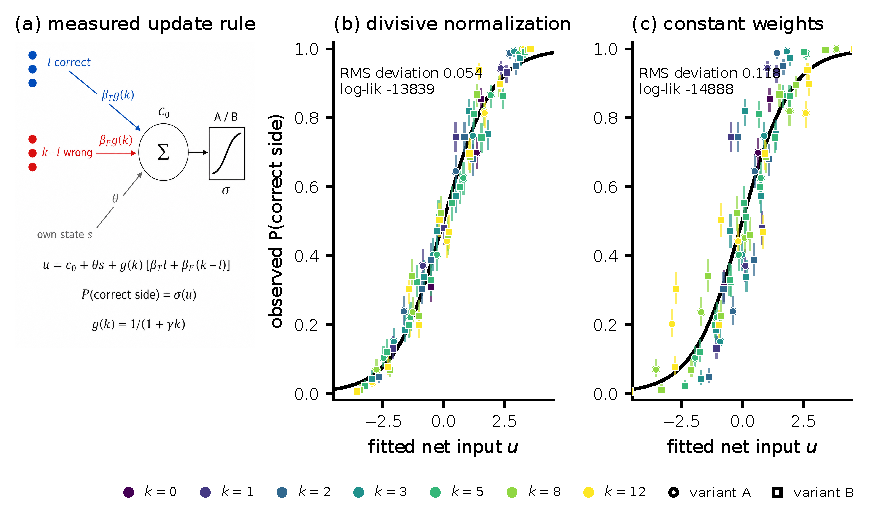
\includegraphics[width=\textwidth]{fig3_neuron}
\caption{\textbf{Observed correct-side rate against fitted net input under divisive and constant message weights.}
(a)~The measured update rule: $l$ correct-side and $k-l$ wrong-side messages
enter with weights $\beta_T g(k)$ and $\beta_F g(k)$, the own-state indicator
$s \in \{0,1\}$ (variant B only) with weight $\theta$, and the field $c_0$;
the choice probability is $\sigma(u)$ with $g(k) = 1/(1+\gamma k)$,
$\gamma = 0.9$. (b)~Observed correct-side rate in each of the 78 design cells
of the 31{,}824 randomized queries (variant $\times$ $k$ $\times$ $l$
$\times$ $s$; 408 queries per cell; Wilson 95\% intervals) against
$u$, the logit of the model's mean predicted probability in the cell
(divisive normalization, claim fixed effects), so that a model calibrated in
that cell places it on the curve $\sigma(u)$. Color gives inbox size $k$;
circles variant A, squares variant B. (c)~The same cells under constant
weights ($g \equiv 1$): large-$k$ cells lie between the curve and 0.5 and
small-$k$ cells beyond it. RMS deviation of cell rates from $\sigma(u)$: 0.054 in
(b), 0.118 in (c).}
\label{fig:neuron}
\end{figure}

\section{Collective experiment}\label{sec:collective}

\subsection{Design (pre-registered before any collective run)}

Networks are generated per episode by the acceptance process at capacity
$\alpha$; initial opinions are assigned exogenously ($\lceil 32 x_0 \rceil$
agents seeded correct-side); dynamics follow El et al.'s protocol --- one
broadcast message per agent per round conditioned on its current stance,
Markovian inboxes, snap-judgement opinion resampling --- for eight rounds. The
main arm (variant A prompts) runs $\alpha \in \{0.20, 0.30, 0.38, 0.45, 0.55,
1.00\} \times x_0 \in \{4,\dots,24\}/32$, adaptively concentrated where $q$
crosses $\tfrac12$ and, above the predicted $\astar$, at low $x_0$ where the
collapse of the wrong basin is most visible. The discrimination arm (variant B
prompts) runs $\alpha \in \{0.60, 0.90, 1.30\}$. A rewiring control
(in-degree-preserving shuffle with rewiring fraction $\rho = 1$, i.e., all sources resampled, at $\alpha = 0.30$) checks
that outcomes are reproducible when every receiver's sources are redrawn at
fixed in-degree, a test of reproducibility under the mean-field premise rather
than of its sufficiency (Section~\ref{sec:results}); a yoked one-step analysis
replays every realized inbox through the Section~\ref{sec:measurement}
response function, so that any collective deviation from iterated single-agent
behavior is measured rather than assumed absent; and a surrogate rollout of
the measured per-$k$ rule on the same graphs and seeds provides the
finite-size prediction band. Decision criteria were fixed in advance: the
empirical $\astar_{\mathrm{emp}}$ is the capacity at which the wrong-consensus
rate from $x_0 \le 8/32$, after eight rounds, falls through 20\%, and the
discrimination arm's verdict is read from which $\alpha$ levels retain a
wrong basin. Outcomes are read after eight rounds: an episode ends in a
correct-side consensus when $x_8 \ge 0.6$ and a wrong-side consensus when
$x_8 \le 0.4$. The threshold is operational; among decided episodes the final
fraction lies beyond $|x_8 - 0.5| > 0.4$ in 63\% of the main arm's episodes
(median wrong-side end state $x_8 = 0.03$) and in 97--99\% of the qwen3:8b
campaigns of Section~\ref{sec:generality}, so the labels describe strongly
polarized end states, and the sensitivity of every result to the threshold
($\delta \in \{0.05, 0.2\}$) is reported in the SI.

\subsection{Results}\label{sec:results}

The pre-registered prediction failed, and we state the failure before its
diagnosis. Across all 1{,}414 episodes (zero parse failures), the
correct-consensus probability never reached 0.5 in any $(\alpha, x_0)$ cell:
the collectives converge on the wrong consensus from most initial conditions,
and even from $x_0 = 24/32$ the correct-side outcome occurred in only
28--45\% of episodes (wrong-side 33--73\%, undecided 0--28\%;
Fig.~\ref{fig:collective}a). The
wrong-consensus rate from low $x_0$ falls monotonically with $\alpha$ --- 0.98
at $\alpha = 0.20$ to 0.75 at $\alpha = 1.00$, the direction the theory
predicts --- but never crosses the pre-registered 20\% threshold, so no
empirical critical crowding level exists in the window: the prediction
$\astar = 0.435 \pm 0.03$ is rejected (claim-clustered bootstrap, 0 of 2{,}000
resamples crossing).

The diagnosis localizes the failure to the wording-induced field. Replaying
every realized inbox through the Section~\ref{sec:measurement} response
function with each claim's own field (per-message weights pooled over the 17
calibration claims, field fitted per claim) reproduces the observed
transitions without systematic error: Brier 0.10--0.14 against 0.17--0.25 for
always predicting the base rate, expected calibration error 0.03, and a
residual of $-0.02$ to $+0.01$ at contested compositions
($l/k \approx \tfrac12$). The four experimental claims, chosen for
near-neutral fields, carry fields of 0.16--0.55 under the scaffold; the
calibration set's fields average 0.94, and the blind rule inherited that
average. Re-inserting the four fields into the unchanged theory predicts the
observed phase: a single wrong-consensus attractor for three claims at every
$\alpha$ in the window ($x^* = 0.02$--$0.11$) and, for the fourth, a wrong
basin extending to $x_0 \approx 0.7$ up to $\alpha = 0.55$. Rolled out for
eight rounds on the realized graphs and seedings, the same rule reproduces
the wrong-consensus rate from low $x_0$ (0.93--1.00 predicted, 0.75--0.99
observed) and the final fractions to an RMS of 0.09 over the 36 cells;
replacing the realized graphs by the mean-field independence assumption
changes the eight-round prediction by a further 0.04 (RMS). We call this
failure mode field transport: a field measured on one claim set does not
carry over to another, whereas the message weights do. A second limit of the
blind test is the horizon. The blind rule's own eight-round surrogate on the
realized graphs falls below 20\% wrong consensus only at $\alpha = 0.63$, not
at $\astar = 0.435$ (at $\alpha = 0.45$ it still predicts wrong consensus in
67\% of low-$x_0$ episodes; Fig.~\ref{fig:collective}a, dashed), so the
pre-registered criterion tested the fold through a horizon that displaces it
by about 0.2 in $\alpha$: the fold is a property of the infinite-time map,
the experiment a statement about eight rounds, and the two are compared
through the surrogate, not directly. The two causes separate on the
counterfactual: with the blind field, the surrogate fails the 20\% criterion
at $\alpha \le 0.55$ on its own (horizon), but at $\alpha = 1.0$ it predicts
wrong consensus in 0.1\% of low-$x_0$ episodes against 75\% observed (field).
The field is why the prediction fails across the window; the horizon is why
the criterion could not have resolved the fold near $\astar$ even with the
right field.

The discrimination arm survives with a weaker verdict
(Fig.~\ref{fig:collective}b). Under the pooled coefficients the constant rule
predicted no wrong basin at $\alpha \ge 0.6$ and the normalized rule
predicted absorption up to $\alpha = 1.3$; wrong-consensus rates of
0.975--1.00 at all three capacities matched the normalized prediction, which
was the pre-registered criterion. With claim-resolved fields, however, both
coupling rules predict wrong-side attractors at these capacities, and the arm
separates them less sharply: the normalized rule places the low-$x_0$ final
fractions at 0.10--0.20 against 0.06--0.10 observed, the constant rule at
0.25--0.39. The data favor the normalized rule but do not reject the constant
one, and one claim (1569) converged wrong-side where both rules predicted
correct-side convergence. Degree-preserving rewiring ($\rho = 1$ at
$\alpha = 0.30$) changed the outcome probability by at most 0.09 in any cell
and by 0.00 in four of six; because the generated network is itself uniform
given its degrees, this control tests reproducibility under redrawn sources
rather than the sufficiency of $P(k)$. One residual remains: the collectives
end slightly more correct than the iterated single-agent rule predicts (final
fractions 0.05--0.17 above the surrogate in 11 of the 12 cells at
$x_0 \ge 5/8$). The collective experiment thus rejects the blind prediction,
verifies each link of the reduction chain except the transport of the field
across claims, and identifies the claim's field as the quantity that
decided the outcome in the main arm.

\begin{figure}[t]
\centering
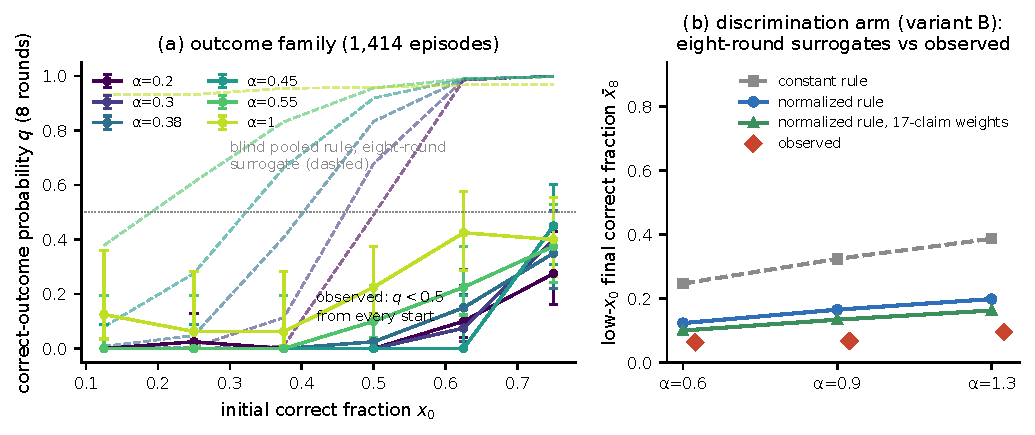
\includegraphics[width=\textwidth]{fig4_collective}
\caption{\textbf{Outcome probability after eight rounds against the surrogate of the pre-registered rule (arm A), and low-$x_0$ final fractions against surrogates of two coupling rules (arm B).}
(a)~Observed outcome family $q(x_0)$ after eight rounds (solid, Wilson 95\%
intervals) against the eight-round surrogate of the blind pooled rule on the
same graphs and seedings (dashed): the blind prediction is rejected; the
correct-side outcome probability stays below 0.5 from every initial
condition. (b)~Discrimination arm:
observed low-$x_0$ final fractions against the eight-round surrogates of the
normalized (divisive) and constant coupling rules with claim-resolved fields;
the normalized rule lies closer, the constant rule is not rejected.}
\label{fig:collective}
\end{figure}

\subsection{What the field is: a pre-registered discrimination experiment}

The dominant field admits three interpretations, which we separated with
predictions registered before data collection: an assertion-polarity bias
(collectives drift toward affirming the claim, whatever its content), a truth
asymmetry (wrong content itself is favored), and a parametric-prior pull
(collectives drift toward the model's stored world knowledge). Two designs
separate them. First, collectives on three \emph{true} claims (labeled SUPPORTS in CLIMATE-FEVER):
polarity and prior predict correct-side convergence, truth asymmetry predicts
wrong-side. Second, collectives on minimally negated rewrites of the four
original misinformation claims --- each rewrite denies what its original
affirms about the same proposition, so that the correct side switches from
denying to affirming; three by inserting a negation and the fourth by
replacing ``a non-problem, or even a benefit'' with ``a problem, and not a
benefit'' (a contrary rather than a strict negation, with the quantifier
``often'' retained), equivalence checked by model judgment and by hand:
polarity predicts the drift reverses with the wording; both alternatives
predict it does not.

The verdict is polarity (Fig.~\ref{fig:polarity}). On all three true claims
the collectives converged on the correct (affirming) side from every initial
condition, including 12.5\% correct starts (mean final fractions 0.67--1.00),
rejecting truth asymmetry. On all four negated rewrites the collectives
converged on the affirming side, which is now the correct side (correct-side
fractions 0.98--1.00), exactly as the originals had converged on the
affirming side when it was the wrong side (correct-side fractions
0.00--0.43): the assertion-referenced outcome is the same, the
content-referenced outcome reverses with the wording, which a
parametric-prior pull fixed by content cannot produce. The parametric-prior
account is thus rejected in the form tested, a content-fixed prior read from
the bare prompt (a quantity that, as Section~\ref{sec:measurement} notes,
does not itself carry over to the full scaffold), not in every conceivable
form. One rewrite whose bare-prompt field pointed to the \emph{denying} side
($p = 0.34$) still converged on the affirming side; this is the one pair in
which field and polarity opposed each other, and the polarity channel
overrode the field rather than merely riding it. Single-agent
predictions again matched the collective outcomes claim by claim in all ten
(claim, $\alpha$) cells, two of them to within the resolution of the seeding
grid (SI). A sender-side account, in which denying messages are simply
weaker text, is excluded by two measurements: the tilt is present with an
empty inbox, before any message is read, and the same 8B-generated message
bank read by llama3.3:70b yields a per-message asymmetry of 1.03
$[0.66, 1.64]$ (Section~\ref{sec:generality}), so the asymmetry travels with
the reader, not with the messages. For this model, the collectives follow
the assertion, not the truth --- which reframes the social reading of Section~\ref{sec:results}: the
collectives lose to misinformation here because misinformation is phrased as
an affirmation, not because wrong content is favored. The same reading bears on
reports that LLM opinion networks converge toward scientific ground truth
regardless of initial stance \citep{Chuang2024}: where the true position is
the affirming one, a polarity channel and a truth bias make identical
predictions, and only designs that reverse the assertion direction --- as
here --- separate them.

\begin{figure}[t]
\centering
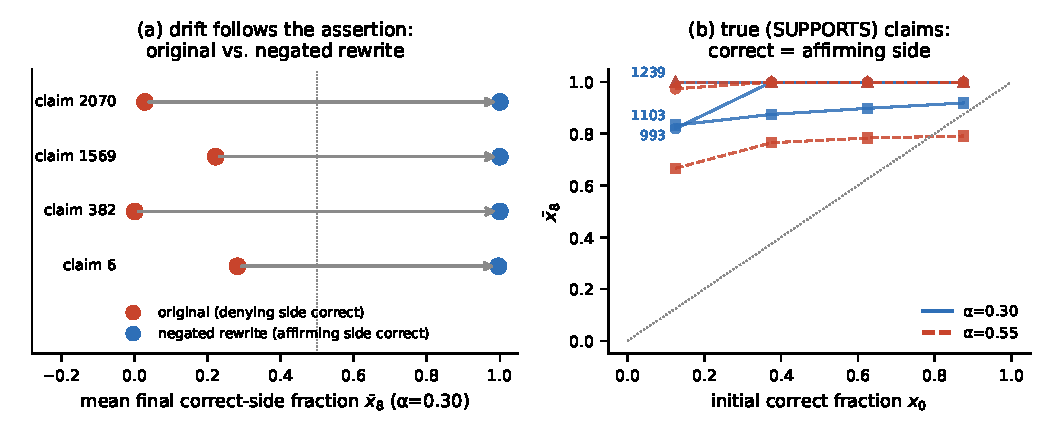
\includegraphics[width=\textwidth]{fig5_polarity}
\caption{\textbf{Final correct-side fractions for original, negated, and true claims.} (a)~Mean final correct-side
fraction for the four original claims (denying side correct) and their
minimally negated rewrites (affirming side correct) under identical
conditions: the content-referenced outcome reverses with the wording.
(b)~True (SUPPORTS) claims converge on the correct = affirming side from all
initial fractions.}
\label{fig:polarity}
\end{figure}

\subsection{The regime is a model property}\label{sec:generality}

Running the identical pipeline --- claim calibration and randomized
single-shot measurement, then collectives, with fixed-point predictions
computed from the single-shot fits alone --- on a second 8-billion-parameter
model (qwen3:8b) produced a
qualitatively different outcome (Fig.~\ref{fig:generality}). For all twelve
qwen3:8b claims the single-agent data were collected before the
corresponding collectives ran; the fixed points reported here are computed
from those data with the final estimation procedure (Methods), so their
agreement with the collectives is an out-of-sample test in which no
collective outcome enters the fit, though not a prospective registration.
The eight-claim campaign below adds the prospective element: its
claim-selection rule was registered before its data existed. For
this model the theory predicts, from the single-agent measurements alone,
claim-dependent bistability: an interior unstable fixed point at 0.14--0.21
for one claim (falling with $\alpha$ and leaving the seeding grid at
$\alpha = 1.0$) and at 0.70--0.71 for another. Both appeared. Collectives
seeded at $x_0 = 0.125$ split between the two basins while every start at
0.375 or above converged correctly; for the second claim the correct-side
outcome probability was at most 0.3 from every start at 0.625 or below (mean
final fractions 0.00--0.42) and 0.9--1.0 from 0.875, placing the observed
crossings at 0.69--0.75. These are the first observed
interior thresholds in this study, at the computed positions. For the
remaining two claims the pipeline predicts monostable correct-side
convergence in every cell but one (the negated rewrite of claim 1569 at
$\alpha = 0.30$, predicted bistable with threshold 0.37), and the collectives
converged correctly in every cell but that one, where the observed crossing
is 0.35 $[0.28, 0.43]$: all twelve cells match in class (one to within the
resolution of the seeding grid), five of six predicted thresholds fall inside
the observed intervals (the sixth misses by 0.02), and the prediction and
observation intervals overlap in all six. This model is also not
assertion-following: one true claim converged to the \emph{denying} side from
all starts below 0.625, which no polarity account permits.

A calibration campaign then took the comparison beyond these four claims.
Twenty further claims were calibrated and measured single-shot; the same
pipeline classified each (claim, $\alpha$) cell --- monostable correct-side,
monostable wrong-side, or bistable with a computed threshold --- eight claims
spanning the predicted regimes were selected by a pre-registered rule applied
to the classifications computed at the time of the campaign (the predictions
reported here, recomputed with the estimation procedure of Methods, leave the
selected claims' classes unchanged in 15 of 16 cells), and
256 further episodes were run ($\alpha \in \{0.30, 0.55\}$, eight initial
fractions, zero parse failures). The predicted classification matched the
observed one in 15 of 16 cells (Fig.~\ref{fig:calibration}). Across the
eleven cells observed bistable, all eleven predicted thresholds fall inside
the episode-bootstrap intervals, the mean absolute difference between
predicted and observed thresholds is 0.04, and the two are rank-correlated at
$r_s = 0.96$ (Spearman; $p = 0.004$ under permutation of claim labels, claims
being the exchangeable unit). Prediction-side uncertainty, from resampling
each claim's single-shot queries, gives intervals of width 0.08--0.25 on the
predicted thresholds that overlap the observed intervals in all eleven cells
(Fig.~\ref{fig:calibration}, horizontal bars). The one mismatch is a claim at
$\alpha = 0.30$ whose predicted threshold, 0.09, lies just above the lowest
seeded fraction ($2/32$), from which its collectives nevertheless converged
correctly; at $\alpha = 0.55$ the same claim's predicted threshold (0.03) and
observed crossing (0.01 $[-0.09, 0.17]$) agree, and it is bistable in only
62\% of the resampled predictions, marking it as the boundary case. What was
an existence proof on two claims is thus a calibration curve on eight: the
single-agent pipeline predicts not only whether a threshold exists but, to
the resolution of the seeding grid, where it sits.

The larger model completes the comparison. In llama3.3:70b, probed at the
single-agent level with the same eight claims and message bank, the
per-message assertion asymmetry is 1.03 $[0.66, 1.64]$, against 1.44
$[1.25, 1.65]$ for llama3.1:8b over the 17 calibration claims and 1.94
$[1.39, 2.73]$ on these same eight (difference 0.90 $[0.00, 1.72]$,
claim-clustered), and the bare fields align with content for seven of the
eight claims (with an empty inbox, $P(\mathrm{TRUE}) = 0.000$ for the four
false originals and $1.000$ for three of the four true rewrites; the eighth,
the negated polar-bear rewrite, is near neutral at $P(\mathrm{TRUE}) = 0.42$):
the polarity channel that governed the 8-billion-parameter collectives is not
detected, and the larger model's collective regime --- not measured here, a
stated limitation --- would be field-dominated on most realistic claims. The
larger model differs from llama3.1:8b in model generation as well as in
scale, so the comparison bounds the channel in the larger model rather than
isolating scale as its cause. Whether a collective has a transition point at all, where it sits, and what
force drives consensus are, across the two models whose collectives were run,
and for the polarity channel in the third, properties measurable on the
individual agent before any collective is run.

\begin{figure}[t]
\centering
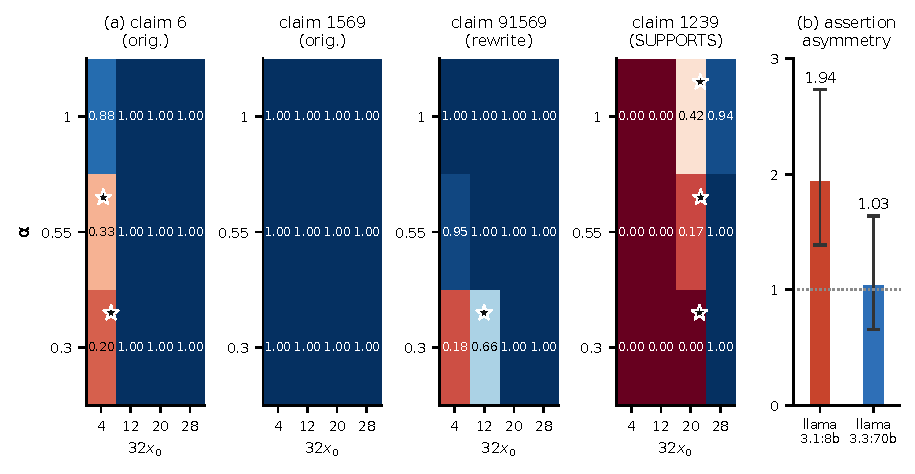
\includegraphics[width=\textwidth]{fig6_generality}
\caption{\textbf{qwen3:8b collective outcomes against predicted fixed points, and the per-message asymmetry at 70B.} (a)~qwen3:8b
collectives: mean final correct-side fraction per cell; stars mark the
predicted unstable fixed points, which coincide with the observed basin
boundaries for claims 6, 1239, and 91569 at $\alpha = 0.30$; claim 1569 is
predicted and observed monostable correct-side. Cell values are mean final
fractions; intermediate values are splits between the two basins, not
intermediate end states (per-cell outcome counts in the SI). (b)~The
per-message assertion asymmetry on the same eight claims and message bank
(claim-clustered 95\% intervals) is not detected at 70B.}
\label{fig:generality}
\end{figure}

\begin{figure}[t]
\centering
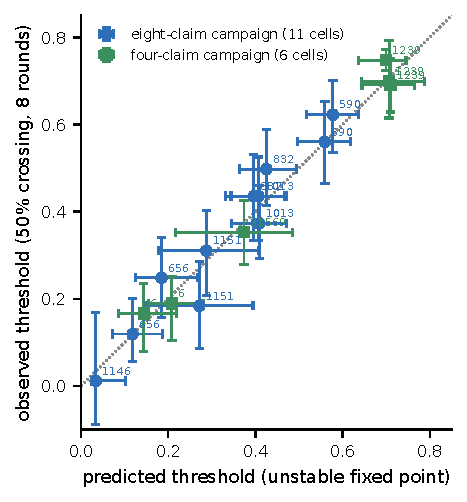
\includegraphics[width=0.72\textwidth]{fig7_calibration}
\caption{\textbf{Calibration of threshold predictions (qwen3:8b).}
Predicted unstable-fixed-point position (per-claim divisive response
function) against the observed threshold (50\% crossing of the eight-round
outcome) for every (claim, $\alpha$) cell observed bistable: circles, the
eight-claim campaign (11 cells); squares, the four-claim campaign (6 cells).
Vertical bars are episode-bootstrap 95\% intervals of the observed
threshold, horizontal bars are single-agent-bootstrap 95\% intervals of the
prediction, and the dotted line is identity. Cells predicted and observed
monostable (4 of 16 and 6 of 12) and the one class mismatch (claim 1146 at
$\alpha = 0.30$) are listed in the SI.}
\label{fig:calibration}
\end{figure}


\section{Discussion}\label{sec:discussion}

The intake budget is a design variable for collective reliability: through
$P(k)$ it sets whether a wrong-consensus basin exists, and the critical
budget $K^*$ is computable from single-agent coefficients through the reduced map ---
on the precondition that the wording-induced field and any model-specific
polarity channel are measured first, since these decide which phase diagram
the budget is operating in. The evidence is three models run against
predictions computed from single-agent measurements alone:
assertion-dominated monostability in llama3.1:8b, where field and polarity
override the budget and 75\%-correct majorities are lost in most episodes; claim-dependent
bistability with predicted thresholds in qwen3:8b (15 of 16 cells); no
detectable polarity at 70B. A blind prediction, its pre-registered rejection,
the replay-based localization of the failure, and the cross-model confirmation of
the pipeline with claim-resolved fields are reported together. Throughout,
the $\alpha$ trend of the wrong-consensus attractor --- observed and
predicted --- shows that the number of messages each agent was actually shown
remained the operative degree even where the blind prediction failed: the
failure mode was the transport of the field across claim sets, not the
identity of the degree.

The blind test carries two lessons for prediction in this setting. The field
must be measured on the claims that will be debated: message weights pooled
over a calibration set transfer, the field does not. And the decision
criterion must be computed for the horizon of the experiment: the fold of the
mean-field map is an infinite-time statement, and near the fold the map
relaxes slowly, so an eight-round experiment must be compared with an
eight-round surrogate rather than with the fold itself. What the collectives
verified should also be stated precisely. The observed transitions are
thresholds in the initial fraction at fixed capacity, at the positions the
pipeline computed. The fold in $\alpha$ itself, the vanishing of the wrong
basin as capacity is reduced, was predicted for llama3.1:8b and not observed,
because the claims' fields placed three of the four claims in the
wrong-side monostable phase at every capacity tested and the fourth in a
bistable phase whose threshold lay near $x_0 \approx 0.7$. The capacity
dependence that was observed is
the movement of the qwen3:8b thresholds with $\alpha$ (claim 6: 0.21 to 0.14
predicted, 0.19 to 0.17 observed, then below the seeding grid at
$\alpha = 1.0$), which is the same fold approached from the side of the
initial fraction. The title's claim is the first of these: capacity sets
where the threshold sits, verified in qwen3:8b, and the wording sets which
phase the collective is in; whether capacity can remove the threshold
altogether, the fold in $\alpha$, is the prediction that llama3.1:8b's fields
kept out of reach.

What $\alpha$ corresponds to outside this experiment differs by system. Here $\alpha$ is an enforced
reading budget: in this protocol the router, not the model, implements the
acceptance kernel, a division of labor the measurements themselves selected
(Section~\ref{sec:measurement}). In deployed multi-agent systems its
counterparts are the quantities that bound how many messages an agent
reads --- finite context windows, per-token costs, and the sampling policies
of agent frameworks; in the naming-game literature the analogous bound is a
finite interaction memory \citep{Flint2026}; in human information sharing,
divided attention limits message visibility in the same direction
\citep{HodasLerman2012}. The model's own capacity enters the theory
separately, as the measured load attenuation $\beta(k)$: the intake budget
sets who is read, the attenuation sets how much each reading counts.

Dialogue does not correct error in the field-dominated phase: majorities of
75\% correct agents ended correct-side in fewer than half of the episodes at
every capacity tested, and the discrimination experiment shows the drive is the assertion,
not the content. Communication volume and capacity are no remedy where the
per-reading tilt is adverse --- a limiting condition on idealized-Bayesian
accounts of collective knowledge \citep{Taniguchi2024}. The
misinformation-vulnerability reading must be stated carefully: small llama
collectives lose to misinformation because misinformation affirms; models
without the polarity channel (qwen, 70B) fail or succeed by different
routes. Directional conformity has likewise been reported to collapse
majority-vote aggregation in LLM safety panels under peer pressure
\citep{HuQu2026}; the polarity channel measured here is a claim-level
analogue that requires no peer opinions at all --- it is present in bare
single-shot calibration.

The origin of the polarity channel is probed and bounded rather than
resolved. An abliterated (refusal-direction-ablated, \citealp{Arditi2024})
derivative of the same instruct model retains the channel --- per-message
asymmetry 1.24 $[1.05, 1.47]$ against 1.44 $[1.25, 1.65]$ for the intact
model, measured in the same batch with the same message bank --- so removing
refusal behavior does not remove the assertion bias, and any reduction is
below this measurement's resolution. Whether the channel exists before
instruction tuning could not be measured: the base model does not follow the
forced-choice format (parse rate below 5\% even with a three-shot format
prefix), which places pre-tuning behavior outside any forced-choice probe; a
log-probability readout is the instrument for that question. The channel is
adjacent to, but not identical with, sycophancy as usually defined ---
agreement with a user's stated opinion, traced in part to the preference
data used for RLHF \citep{Sharma2023}; here the agreement is with the
claim's own assertion, with no user opinion in the prompt. What can be said
is negative and useful: the bias that decides these collectives' fate is not
carried mainly by the safety-refusal direction.

Two further single-agent observations are recorded without mechanistic
claims: opinion flips concentrate in particular agents rather than being
suppressed after a flip (a positive ``anti-refractory'' coefficient,
$+0.98$), and the measured branching ratios (1.8--3.6) place these
synchronous dynamics in a drift-dominated, far-from-critical regime ---
closing, for now, a self-organized-criticality reading of these collectives.

What is verified here is the reduction chain from single-agent response and
degree statistics to the basin boundaries of \emph{LLM} collectives at fixed
capacity; the fold in capacity itself remains a theoretical prediction.
The suggestion for human groups is nonetheless concrete. The cognitive limits cited in the Introduction give human participants a finite effective intake of the same shape, and the theory's inputs (response tilt, load attenuation, intake bound) are all behavioral, none tied to a machine substrate. If deliberating groups sit at finite effective $\alpha$, the theory would say which of them can recover the truth from a correct minority and which cannot. Statements about human collectives are implications, not measurements:
locating a human group on the computed $\astar$ curve would need, besides an
estimate of a human $\alpha$ from intake-saturation data, the human
counterparts of the response coefficients (the tilt, the per-message weights,
and their load attenuation), none of which is measured here. A further limitation is the
REFUTES-skew of the calibrated claim set, which restricts all claims to
correct-side/wrong-side language; identifying genuine truth asymmetry needs
a claim set balanced in polarity at matched difficulty, which this model's
one-sided accuracy on SUPPORTS claims may make impossible --- with the
mitigation that the $\astar$ prediction never invoked truth asymmetry: the
theory weights correct-side and wrong-side messages by their measured
coefficients, and the measured inequality $|\beta_T| \ne |\beta_F|$
($\delta < 0$) is, for this REFUTES-skewed set, the assertion asymmetry seen
from the correct side, not a truth asymmetry.

Relative to \citet{El2026}, their graphs were given, ours are generated;
their fits describe the collective data, ours are computed from single-agent data alone. The two studies probe
orthogonal axes of one phase diagram for the same class of system --- binary
units with logistic (Glauber-type) updates. Their transition is thermal:
topology fixed, noise swept, a critical point located by a susceptibility
peak, on symmetric couplings that admit an energy function. Ours is
topological: effective noise fixed (absorbed in the measured $\beta$),
degree statistics swept through $\alpha$, and the transition is a fold ---
the disappearance of a metastable basin, a spinodal rather than a critical
point, which is why the collapse of the wrong basin and not a fluctuation peak is the
correct observable. Our graphs are directed, so the dynamics are non-equilibrium and free-energy arguments do not transfer; the mean-field
map does. Model-dependent collective regimes have now been reported in the
coordination setting as well --- naming-game populations whose collective
bias amplifies, induces, or reverses individual bias with model-specific
size thresholds \citep{Flint2026} --- convergent with the model dependence
measured here; and the structured interaction topologies those authors list
as future work are what the crowding process supplies. For
consensus-scaling observations \citep{DeMarzo2024},
$(\log N)/\alpha$ supplies the analytic form for the reported size-limited
consensus.

Part of the logistic form is guaranteed by the output mechanism: for a
forced choice between two options, the probability of one option conditional
on the answer being one of the two, $P(A \mid A\ \text{or}\ B) =
\sigma((z_A - z_B)/T)$, is exactly a logistic function of the logit
difference at temperature $T$; the response format asks for a single
character and parse failures were zero in every collective campaign, so the
measured choice probabilities are close to this conditional quantity. What the mechanism does not guarantee --- the
empirical content of the reduction --- is that this logit difference is
approximately additive in the inbox composition, one weight per
correct-side and per wrong-side message (Fig.~\ref{fig:neuron}b). Additivity in log-odds is what an
aggregator of conditionally independent evidence would produce; whether
the transformer approximates such a computation, and why, is left open
alongside the mechanism of the attenuation below.

The measured update rule (Fig.~\ref{fig:neuron}a) departs from a classical Ising spin in exactly one
place: the per-message coupling is attenuated by the total inbox size,
$\beta/(1+\gamma k)$, the form known in sensory neuroscience as divisive
normalization \citep{CarandiniHeeger2012}. As in that literature, the law is
phenomenological --- a behavioral input--output relation, not an identified
mechanism. Three candidate mechanisms make separable predictions: softmax
attention inside the transformer is itself a divisive operation, and
predicts attenuation governed by token volume rather than message count;
proportion coding --- judging by the fraction $l/k$ of supporting messages
rather than their number, the saturation pattern classically reported for
human majority influence --- predicts dependence on $l/k$ alone; and
calibration compression of the output probabilities would mimic attenuation
and is excluded or quantified by reading log-probabilities directly. A
factorial manipulation of message length and proportional $(l, k)$ scaling
within the Section~\ref{sec:measurement} protocol would separate the three;
we leave this as a stated open question, since no result in this paper
depends on which mechanism generates the measured form.

The practical rule this work supports is short: measure the tilt first, then
set the budget. Both are single-agent measurements, and together they
account for most of what the collectives did, with residuals of 0.05--0.17 in
final fraction and one claim outside both coupling rules remaining. The
residual is small but systematic (11 of 12 cells, same sign), so it measures
a collective contribution beyond the iterated single-agent rule rather than
noise. One candidate is the evolution of message content across rounds: the
influence of correct-side messages grows by $+0.026$ per round in the
one-step regression (SI), which could reflect either the messages or repeated
exposure. Replaying single-shot queries with round-specific message banks
built from the logged episodes would separate the two; the logs permit it.

\section*{Methods}

\subsection*{Models and serving}

All agents are served with ollama. The primary model is llama3.1:8b
(Q4\_K\_M quantization, temperature 0.7 throughout, seed recorded for every
call). The cross-model campaign uses qwen3:8b (tag 500a1f067a9f, thinking
disabled via \texttt{think:false}) and llama3.3:70b (Q4\_K\_M; judgments
only, message banks fixed to the 8B-generated banks). Single-shot campaigns
ran against a user-space ollama instance with \texttt{OLLAMA\_NUM\_PARALLEL=16}
(the system instance saturates at 0.62 generations/s; the parallel instance
reaches 3.5 generations/s); the 70B model does not load under 16-slot KV
allocation and was served by the serial system instance. The polarity-origin probe (Discussion) used two further variants, judgments
only: llama3.1:8b-text-q4\_K\_M (the base model) and an abliterated derivative
of the instruct model (mannix/llama3.1-8b-abliterated, Q4\_0), with a
three-shot answer-format prefix applied identically to all variants,
including the re-measured instruct control. Every call's prompt
hash, seed, raw response, and parse result are logged to JSONL.

\subsection*{Prompts}

The judgment prompt (verbatim; variant A) is:
\begin{quote}\footnotesize\ttfamily
\# Your Expertise\\
\{persona\}\\[2pt]
\# Messages\\
You received the following messages from fellow panelists:\\
- \{message 1\} \ldots\\[2pt]
\# Problem\\
You are one member of an expert panel judging the following claim.\\
Claim: "\{claim\}"\\
Options:\\
A) \{TRUE or FALSE\}\\
B) \{FALSE or TRUE\}\\
\# Instruction\\
Give your direct answer on which option is correct.\\
Do NOT work through the problem, show any steps, compute, or\\
explain --- just commit to a snap judgement.\\
\#\# Response Format\\
Respond with a single character, A or B, and nothing else.
\end{quote}
Variant B inserts, before \texttt{\# Problem}: ``\texttt{\# Your Current
Answer / Your current answer is that the claim is \{TRUE|FALSE\}.}'' The A/B
$\leftrightarrow$ TRUE/FALSE assignment is randomized per call and
counterbalanced within cells; message presentation order is randomized and
recorded. The message-generation prompt asks the sender, given its persona,
the claim, and its current stance, to ``write a brief message to a fellow
panelist stating that you believe the claim is \{stance\} and giving the
single strongest reason from your reasoning,'' with a two-sentence response
format; stance is expressed in the message body (TRUE/FALSE), never as an
option letter, because option labels are randomized per receiver. Personas are
one-line expertise statements drawn from a fixed pool of 12. Prompt texts are
extracted verbatim from the released scripts.

\subsection*{Claims and calibration}

Claims are drawn from CLIMATE-FEVER \citep{Diggelmann2020} (SUPPORTS and
REFUTES only; the claim text is presented alone, without evidence). A
two-stage calibration (24 calls per candidate, refined to 64 for candidates
with $p_q \in [0.35, 0.65]$; A/B assignment counterbalanced) measured
per-claim accuracy $p_q$ and field $h_q = \mathrm{logit}(p_q)$. The collective
experiments use per-claim fields re-estimated under the full experimental
scaffold (Section~\ref{sec:measurement}). The negated rewrites of the four
Stage-2 claims (each rewrite denies what its original affirms about the
same proposition; three by inserting a negation, one by replacing ``a non-problem, or even a
benefit'' with ``a problem, and not a benefit'', a contrary that avoids a
double negative and retains the quantifier ``often'') were checked for
semantic opposition by model judgment
(70--85\% of 20 counterbalanced calls per pair) and approved by hand before
any collective run. Full claim texts, rewrites, and calibration values are in
the SI.

\subsection*{Networks, episodes, and controls}

Each episode generates a fresh directed network: every receiver processes the
other 31 agents in an independent uniformly random order, accepting the next
candidate with probability $e^{-\alpha r}$ after $r$ acceptances. Initial
stances are assigned exogenously to a uniformly random subset of
$\lceil 32 x_0 \rceil$ agents. Each of eight rounds consists of a message
phase (every agent with at least one out-edge generates one two-sentence
message conditioned on its current stance, broadcast to all its receivers)
and a judgment phase (each agent answers the snap-judgement prompt with its
current-round inbox; single sample). The network is fixed within an episode
(regenerated only between episodes), so a receiver reads the same senders in
every round, and their states are correlated through the shared graph even
though every message is regenerated each round from its sender's current
stance; the independence assumption of the mean field of
Section~\ref{sec:theory} is therefore an approximation. Its cost is
quantified in Section~\ref{sec:results} by comparing the eight-round
iteration of the mean-field map with surrogate rollouts of the same rule on
the realized graphs (RMS difference 0.04 in the final fraction). A fidelity check re-ran ten episodes
with five-sample majority voting; absorption was sharper (wrong-consensus
rate 1.00 versus 0.875, mean $|x_8 - 0.5|$ 0.44 versus 0.38), so the
single-sample simplification is not the source of wrong-side absorption. The rewiring control resamples each receiver's sources uniformly
while preserving its in-degree. Outcomes are classified at $\delta = 0.1$
(correct consensus: $x_8 \ge 0.6$; wrong: $x_8 \le 0.4$), with
$\delta \in \{0.05, 0.2\}$ and undecided-exclusion sensitivity analyses in
the SI.

\subsection*{Cross-model calibration campaign}

Twenty further CLIMATE-FEVER claims (ten SUPPORTS, ten REFUTES, disjoint from
all earlier sets) were calibrated under the full scaffold and measured
single-shot with qwen3:8b (24 calls per candidate, 64 in the boundary band;
per-claim response-function fits from 6{,}720 further queries). The resulting
fixed-point classifications and thresholds for $\alpha \in \{0.30, 0.55\}$
were computed at the time of the campaign, and eight claims were selected by
a rule fixed in the pre-registered instructions (at least four predicted bistable with interior
thresholds, the remainder monostable, filled from the bistable pool where a
category was empty --- no wrong-side-dominant claim existed among the twenty
candidates). Collectives ran the full grid $\alpha \in \{0.30, 0.55\} \times
x_0 \in \{2, 6, \ldots, 30\}/32$ with two replicates (256 episodes, protocol
identical to the main cross-model campaign). Observed thresholds are defined
under Statistics.

\subsection*{Statistics}

All confidence intervals on measured coefficients are claim-clustered pairs
bootstrap percentiles (1{,}000--2{,}000 resamples for the pooled
coefficients, 200 for the identified per-$k$ coefficients and for the
prediction-side intervals, 2{,}000 for the polarity ratios; claims are the
clusters because episodes within a claim share its field). Attenuation-form comparison
uses five-fold cross-validation with folds split by claim, alongside AIC; the
form parameter ($\gamma$ for divisive normalization, the rate for load decay)
is profiled on the full data ($\gamma = 0.9$) and re-profiled inside each
training fold, and a held-out claim's fixed effect, which cannot be estimated
from the training folds, is set to zero, so the cross-validated likelihood
scores prediction for an unseen claim with an unknown field. The divisive
$\astar$ of Section~\ref{sec:measurement} uses $\gamma$ profiled separately
per variant (0.53 for A, 1.32 for B); Fig.~\ref{fig:neuron} uses the pooled
$\gamma = 0.9$. Per-$k$ coefficients are identified by a joint logistic fit
over all inbox sizes with claim fixed effects anchored by the empty-inbox
cells: at a single $k$ the columns $1$, $l$, and $k - l$ are collinear, so
separate per-$k$ fits identify only $c_0 + k\beta_F$ and $\beta_T - \beta_F$.
Per-claim response functions for the collective claims use the reduced form
$c_0 + g(k)[\delta k + \bar\beta(2l - k)]$ ($+\theta s$ for variant B), with
a weak ridge penalty ($10^{-3}$) where $k$ takes three values. For Fig.~\ref{fig:neuron}, one logistic fit per prompt variant
with claim fixed effects and message weights $\beta_T g(k)$, $\beta_F g(k)$
(divisive, $\gamma = 0.9$ fixed, or $g \equiv 1$) assigns each query a
predicted probability; a design cell's net input $u$ is the logit of its mean
predicted probability, and its observed correct-side rate is plotted against
$u$ with a Wilson 95\% interval. Fixed points of the mean-field map are
bracketed on an endpoint-inclusive grid of 4{,}001 points in $x$ with
bisection refinement and classified by $|F'(x)| < 1$; a phase is bistable
when an unstable interior point separates two stable ones, and $\astar$ is
located by bisection in $\alpha$ on that classification, with the fold of $G$
solved jointly from $G = x$ and $G_x = 1$. Prediction-side intervals resample
each claim's single-shot outcomes within that claim and within each design
cell (200 resamples; a within-claim bootstrap, not the claim-clustered
bootstrap used for pooled coefficients) and recompute the fixed points. Reanalysis statistics on the public dataset use
question-clustered bootstrap and CR0 sandwich errors.

\emph{Outcome and threshold.} An episode's outcome is its correct-side
fraction after eight rounds, $x_8$; $q(x_0)$ is the fraction of episodes with
$x_8 \ge 0.6$, a finite-horizon quantity that we compare with the
infinite-time fixed points only through surrogate rollouts. Observed
thresholds are the 50\% crossings of a logistic fit of the correct outcome on
$x_0$ with a weak ridge penalty (0.002) so that separated cells have a
finite estimate; the slope is not constrained, a fit with a non-positive slope
would be discarded, and none occurred in the reported cells. Intervals are
episode-bootstrap percentiles (500 replicates); replicates without a finite
crossing in $(-1, 2)$ are dropped, which retained all replicates in 12 of the
17 cells observed bistable, 97--99\% in three, and 89\% and 65\% in the two
cells whose crossing lies nearest the lowest seeded fraction (claims 656 and
1146 at $\alpha = 0.55$). Rank correlations between predicted and observed thresholds are
tested by permuting claim labels, claims being the exchangeable unit.

\subsection*{Pre-registration timeline}

Throughout this paper, ``pre-registered'' means that a prediction or a
decision rule, together with the criteria for judging it, was written to a
file before the corresponding data were collected, and that the file's
timestamp and SHA-256 hash are recorded in the project repository, so that
the order of prediction and data is documented; these are local records, not
a third-party time stamp. No external registry (such as OSF) was used. Three items were
pre-registered: (i)~the $\astar = 0.435 \pm 0.03$ prediction and the decision
criteria of the main collective experiment, before any collective episode
(2026-08-23); (ii)~the three-hypothesis prediction table of the polarity
discrimination experiment, before its data collection (2026-08-25);
(iii)~the claim-selection rule of the eight-claim calibration campaign,
written into the campaign instructions before its data were collected
(2026-08-27). The single-agent measurements preceded the collective
experiments. The claim-resolved predictions of
Sections~\ref{sec:results}--\ref{sec:generality} were computed after the
collective experiments, with the estimation procedure described under
Statistics, using only the single-agent data for parameter fitting; they were
not prospectively registered. The one adaptive element (second-pass allocation of episodes)
followed rules fixed in the pre-registered design.

\subsection*{Use of generative AI}

The author used Anthropic's Claude for code generation and debugging,
execution of the pre-specified experiment pipelines, drafting and editing of
text, and literature search. The research questions, theory, experimental
designs, pre-registered predictions, and interpretations are the author's;
all AI-assisted output was reviewed and fact-checked, and every reported
number is recomputed from the logged data by the scripts in the public
repository. The language models studied here (llama3.1:8b, qwen3:8b,
llama3.3:70b) are the subject of the research, not writing tools.

\subsection*{Data and code availability}

All episode logs (stance histories, full message texts, graphs, seeds, prompt
hashes), single-shot logs, analysis scripts (scripts 50--57 produce every
identified fit, fixed point, surrogate rollout, and figure reported here), and
notebooks are retained in the project repository, to be released publicly on GitHub
(\url{https://github.com/dockmfgit/AI_agent_crowding}); the public
dataset of \citet{El2026} is not redistributed and is available from its
original source \citep{El2026data}. Layout: \texttt{scripts/} (measurement, engines, analysis),
\texttt{results/} (all tables backing the figures), \texttt{data/}
(raw JSONL and episode JSON), \texttt{notes/} (working records including the
pre-registration files).

\bibliographystyle{plainnat}
\bibliography{refs}

\end{document}
